\section{Additional Details}
\label{app:addition_details}

\paragraph{Dataset Examples.} We list links to dataset sources for our user-provided context in~\pref{tab:context_link_example}.

\paragraph{GPT-4 User's Edits} We list examples of OUR GPT-4 user's edits with different latent preference on summarization in~\pref{tab:user_edits}.

\paragraph{GPT-4 User Template.} Prompt templates used by our GPT-4 user are provided in~\pref{tab:ai_user_prompt_template}.

\paragraph{\algname~Templates.} Prompt templates used by~\algname~are provided in~\pref{tab:agent_prompt_template}.

\paragraph{ICL-edit Templates.} Prompt templates used by \textit{ICL-edit} baseline are provided in~\pref{tab:icl-pref_prompt_template}.

\section{Additional Analysis}
\label{app:additional_analysis}

\paragraph{Detailed Expense Analysis.} We list a detailed computational expense of different methods in~\pref{tab:expense_breakdown}.

\paragraph{Failure Cases.} We summarize our failure case analysis of~\algname~on summarization in~\pref{tab:failures}.

\paragraph{Retrieval Accuracy.} We calculate retrieval accuracy for ~\algname~as the fraction of all retrieved
contexts that are of the same document type as the currently given context across all seeds and time steps.  We report the results in~\pref{tab:retrieval_acc}. We find that the retrieval accuracy is higher on the summarization task than on email writing. and using MPNET typically performs better than using Bert to encode context.






\begin{table}[h!]
    \centering \small
    \caption{Link to each source dataset, from which we randomly sample examples as the user-provided context in our tasks.} 
    \setlength{\tabcolsep}{0.01\linewidth}
    \begin{tabular}{p{0.3\linewidth} p{0.67\linewidth}}
        \toprule
        \textbf{Data Source} & \textbf{Link and Example} \\
        \midrule
        CNN Daily Mail \citep{see-etal-2017-get} & \url{https://huggingface.co/datasets/cnn_dailymail} \\
        SLF5K  \citep{Stiennon2020LearningTS} & \url{https://huggingface.co/datasets/JeremyAlain/SLF5K} \\
        Wikidump  \citep{wikidump} & \url{https://huggingface.co/datasets/wikipedia} \\
        Arxiv \citep{clement2019arxiv} & \url{https://huggingface.co/datasets/CShorten/ML-ArXiv-Papers} \\
 
        IMDb \citep{maas-EtAl:2011:ACL-HLT2011} & \url{https://huggingface.co/datasets/imdb}  \\
        PaperTweet \citep{Bar_PaperTweet} & \url{https://huggingface.co/datasets/nitsanb/paper_tweet} \\
         Elsevier OA CC-By \citep{Kershaw2020ElsevierOC} & \url{https://huggingface.co/datasets/orieg/elsevier-oa-cc-by} \\
 
        \bottomrule
    \end{tabular}   
    \label{tab:context_link_example}
\end{table}


\begin{table}[h!]
    \centering \small
    \caption{Examples of user edits with different latent preference on summarization. The agent output column shows the agent generation without conditioning on any preference. The latent preference for the user edits is in bold and parenthesis. We truncate some examples due to limited space. }
    \begin{tabular}{p{0.45\textwidth} p{0.45\textwidth}}
        \toprule
        \textbf{Agent Output}  & \textbf{User Edits} \\
        \midrule
Leon Fenner, the suspected gunman in a \$2 million diamond heist at Watch Standard Jewelry in New York City, was arrested in Maryland. The robbery occurred on November 11 and resulted in the injury of the store owner's elderly father. Fenner's accomplice, Rondu Frisby, was a friend of the store owner and was apprehended a week after the heist. The robbery took place during the city's Veteran's Day Parade, leading to a block shutdown. Fenner and Frisby stole numerous jewels and 20 luxury watches, but were caught on surveillance cameras. Fenner is set to appear before a federal court in Maryland. 
& \textbf{(targeted to young children, storytelling, short sentences, playful language, interactive, positive)} \newline
Once upon a time in the big, bustling city of New York, during a parade filled with music and marching on Veteran's Day, something sneaky happened at a place called Watch Standard Jewelry. This wasn't just any store; it was a treasure chest full of sparkling diamonds and shiny watches that could make your eyes twinkle like stars.

Now, two not-so-nice men, Leon Fenner and his buddy Rondu Frisby, thought they could be sneaky and take these treasures without asking. On November 11, while everyone was watching the parade, they tiptoed into the store. But oh no! They accidentally hurt the store owner's dear old dad, which wasn't very kind at all.
\textit{[TRUNCATED]} \\



\midrule
The article describes a situation where a neighbor's cat, one of seven rescued by a "cat lady," has started frequenting the author's front yard after leaving its original home due to the presence of other cats. Over the past few months, the cat has become more consistent in its visits, meowing at the author and their family members for attention. The cat allows itself to be petted and shows affectionate behavior, such as rubbing against legs and headbutting hands, until it is fed. After eating, the cat typically leaves but returns in the evening. The author is seeking advice on how to handle the situation, expressing concern about feeding the cat because it is not legally theirs and there could be potential ownership and legal issues.
& \textbf{(second person narrative, brief, show emotions, invoke personal reflection, immersive)} \newline
Imagine yourself in a quaint neighborhood, where the gentle purrs of a feline friend have become a familiar part of your daily routine. This isn't just any cat—it's one of seven, a charming escapee from the home of a local ""cat lady,"" seeking solace in the tranquility of your front yard. Over recent months, this whiskered wanderer has turned your doorstep into its personal stage, meowing for attention with a persistence that tugs at your heartstrings.

Each encounter with this affectionate creature is a dance of mutual admiration. You find yourself captivated by its soft fur and the way it eagerly rubs against your legs, headbutting your hands in a silent plea for affection.
\textit{[TRUNCATED]} \\

\midrule

The Puerto Plata Province is a northern province in the Dominican Republic, known for its beautiful beaches and as a popular tourist destination since the late 1990s. Its capital is San Felipe de Puerto Plata, named after the silver clouds Columbus saw on a mountain nearby in 1493. The city of Puerto Plata was founded in 1502.

Historically, the first European town in the Americas, La Isabela, was established by Columbus near Puerto Plata in 1493. In 1605, the governor Antonio de Osorio destroyed Puerto Plata and other towns to curb illegal trade, leading to the formation of new settlements.

Puerto Plata became a Maritime District in 1865 and was later recognized as a province in the 1907 constitution. Over time, it expanded to include more municipalities and municipal districts, with the latest additions in 2007.
\textit{[TRUNCATED]} 




    & \textbf{(bullet points, parallel structure, brief)} \newline
- Location: Northern Dominican Republic \newline
- Capital: San Felipe de Puerto Plata \newline
- Founding: 1502 by Europeans\newline
- Historical site: La Isabela (1493, first European town in the Americas)\newline
- 1605: Destruction by Governor Antonio de Osorio to stop illegal trade\newline
- Status: Became Maritime District in 1865, recognized as province in 1907\newline
- Expansion: Added more municipalities, latest in 2007\newline
- Borders: Atlantic Ocean, Espaillat, Santiago, Valverde, Monte Cristi provinces\newline
\textit{[TRUNCATED]} \\
\midrule
\end{tabular}
    \label{tab:user_edits}
\end{table}
\begin{table}[h!]
    \centering \small
    \begin{tabular}{p{0.45\textwidth} p{0.45\textwidth}}
        \midrule

The article discusses the challenge of detecting and classifying stuttered speech, which affects many people but has been subject to limited research. The authors present a new model that differs from most existing methods, which typically use language models for stutter identification. Instead, their model is based on acoustic features, which allows it to identify various kinds of stuttering disfluencies without relying on speech recognition technology. The proposed model combines a deep residual network with bidirectional long short-term memory (LSTM) layers to classify different stutter types. It has been shown to significantly outperform current leading methods, reducing the average miss rate to 10.03\%, which is a 27\% improvement over the state-of-the-art.
& \textbf{(tweet style, simple English, inquisitive, skillful foreshadowing, with emojis)} \newline 
Ever struggled with stuttering or know someone who does? 
\includegraphics[height=10pt]{graphs/speaker.png} Research on detecting stutters hasn't been huge, but guess what? A new study is changing the game! 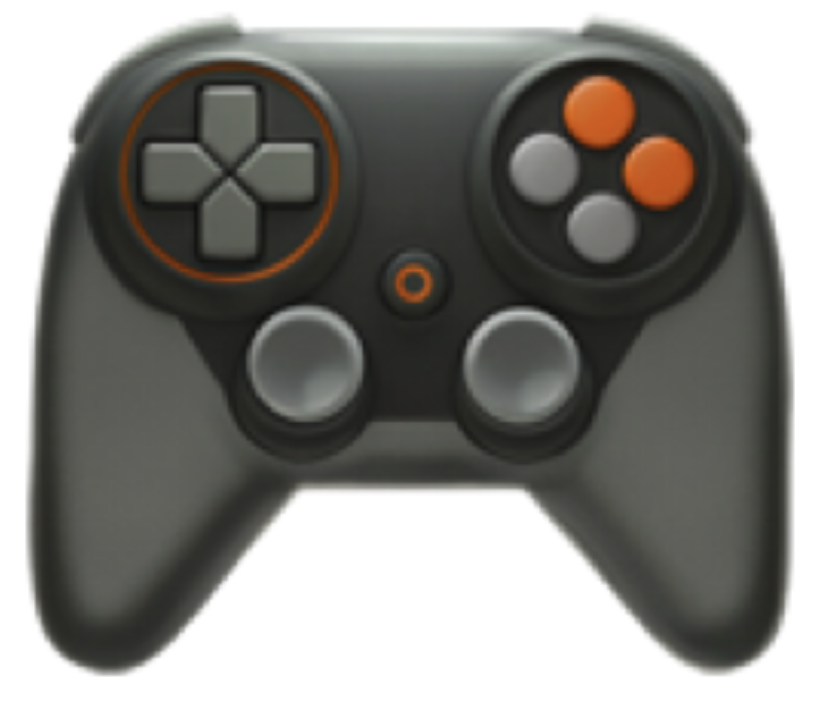
\includegraphics[height=10pt]{graphs/game.png} Instead of just looking at words, this smart model listens to how things are said. 
\includegraphics[height=10pt]{graphs/headphone.png} It's like a detective for sounds, using cool tech called deep learning and memory networks to spot different stutter types. 
\includegraphics[height=10pt]{graphs/detective.png} And it's crushing it, beating old methods by 27\%! Missed stutters? Down to just 10\%! 
\includegraphics[height=10pt]{graphs/chart.png} This could be a big deal for speech therapy! 
\includegraphics[height=10pt]{graphs/hands.png} \#Stuttering \# SpeechTech \# Innovation \\
\midrule
The article discusses a movie that begins promisingly but later becomes confusing due to a poorly depicted portrayal of ancient black magic rituals. The male lead delivers a strong performance despite his character's unfavorable outcome in the climax. The movie is compared to a mix of "Boomerang" and "Extremities."
    & \textbf{(question answering style, direct, concise)} \newline
What is the general sentiment of the article about the movie?

The article suggests that the movie starts off well but eventually becomes muddled. The depiction of ancient black magic rituals is criticized for being confusing.

How does the article describe the male lead's performance?

The male lead's performance is described as strong, even though his character does not have a favorable outcome in the climax.

What films is the movie compared to in the article?

The movie is compared to ""Boomerang"" and ""Extremities"" in the article. 
\\






















































        \bottomrule
    \end{tabular}
\end{table}


\begin{table}[h!]
\centering \small
\caption{Prompt templates for the AI user. The first step is to prompt the user for yes/no answer regarding satisfaction. If the answer is no, the second step is to ask the user edit the agent output according to the latent preference. If the answer is yes, the agent output receives 0 edits.}
\begin{tabular}{p{0.07\linewidth} p{0.4\linewidth} p{0.44\linewidth}}
\toprule
     & \textbf{Summarization} & \textbf{Email Writing} \\
\midrule
    Step 1
    & Article: \context{\{user-provided article\}} \newline
        Summary: \response{\{agent-generated summary\}} \newline
        Is the above summary of the above article good for person who would love to use the following style: \preference{\{latent user preference\}}? Please answer yes or no. 
    & Notes: \context{\{user-provided notes\}} \newline
        Email: \response{\{agent-generated email\}} \newline
        Is the above email based on the above notes good for a user who wants the following style: \preference{\{latent user preference\}}? Please answer yes or no. \\
\midrule
    Step 2
    & Summary: \response{\{agent-generated summary\}}  \newline
        Please revise the above summary of an article to meet your style: \preference{\{latent user preference\}}. 
    & Email: \response{\{agent-generated email\}}  \newline
        Assume that you prefer \preference{\{latent user preference\}}. 
        Please revise the above email to meet your style. \\
\bottomrule
\end{tabular}
    \label{tab:ai_user_prompt_template}
\end{table}


\begin{table}[h!]
\centering \small
\vspace{-10pt}
\caption{Prompt templates for CIPHER.}%
\begin{tabular}{p{0.12\linewidth} p{0.42\linewidth} p{0.42\linewidth}}
\toprule
     & \textbf{Summarization} & \textbf{Email Writing} \\
\midrule
    Task prompt conditioned on inferred preference \newline (\pref{line:generate} in~\pref{alg:cipher})
    & Article: \context{\{user-provided article\}} \newline
        Assume that you need to summarize the above article for a user, 
        who prefers the following style: \preference{\{inferred user preference\}}. 
        Please write a summary of the above article to address those specified preferences.
    & Notes: \context{\{user-provided notes\}} \newline
        These notes are written by a user who prefers the following style of emails: \preference{\{inferred user preference\}}. 
        Please write a short email based on the above notes to address those specified preferences. \\
\midrule
Prompt to infer user preference based on revision \newline (\pref{line:infer_preference} in~\pref{alg:cipher})
    & Original summary of an article: \response{\{agent-generated summary\}} \newline
        Revised summary by a user: \revision{\{user revision\}} \newline
        Based on the edits and revision by this user on the original summary in the above examples, 
        what do you find about this user's generic preference in terms of writing style and formatting?  
        Please answer in a short phrase and only recommend those preferences that are widely used.
    & Original email: \response{\{agent-generated email\}} \newline
        Revised email: \revision{\{user revision\}} \newline
        Based on the edits and revision by this user on the original email in the above examples, 
        what do you find about this user's generic preference in terms of writing style and formatting?  
        Please answer in a short phrase and only recommend those preferences that are widely used. \\
\midrule
    Prompt to consolidate inferred preferences from history \newline (\pref{line:merge_preferences} in~\pref{alg:cipher})
    & List of user preferences successfully being used to generate summaries of similar documents: \newline
        - \preference{\{inferred preference in a retrieved example\}} \newline
        - \preference{\{inferred preference in a retrieved example\}} \newline
        ... \newline
        Based on the the above examples, please come up with short phrase with the most represented summarization preferences of the user. 
    & List of user preferences successfully being used to generate emails of a similar kind: \newline
        - \preference{\{inferred preference in a retrieved example\}} \newline
        - \preference{\{inferred preference in a retrieved example\}} \newline
        ... \newline
        Based on the the above examples, please come up with short phrase with the most represented writing preferences of this user. \\
        
\bottomrule
\end{tabular}
    \label{tab:agent_prompt_template}
\end{table}

\begin{table}[h!]
\vspace{-10pt}
\centering \small
\caption{Prompt templates for the \textit{ICL-edit} baseline.}
\begin{tabular}{p{0.12\linewidth} p{0.42\linewidth} p{0.42\linewidth}}
\toprule
     & \textbf{Summarization} & \textbf{Email Writing} \\
    \midrule
    Prompt with retrieved user edit examples
    & Original summary of an article: \response{\{agent-generated summary in a retrieved example\}} \newline
        Revised summary by a user: \revision{\{user revision in a retrieved example\}} \newline
        Original summary of an article: \response{\{agent-generated summary in a retrieved example\}} \newline
        Revised summary by a user: \revision{\{user revision in a retrieved example\}} \newline
        ... \newline
        Article: \context{\{user-provided article\}} \newline
        Based on the edits and revision by this user on the original summary in the above examples, 
        Please summarize the above article:
    & Original summary of an article: \response{\{agent-generated summary in a retrieved example\}} \newline
        Revised summary by a user: \revision{\{user revision in a retrieved example\}} \newline
        Original summary of an article: \response{\{agent-generated summary in a retrieved example\}} \newline
        Revised summary by a user: \revision{\{user revision in a retrieved example\}} \newline
        ... \newline
        Notes: \context{\{user-provided notes\}} \newline
        Based on the edits and revision by this user on the original email in the above examples, 
        Please write an email based on the above notes for this user: \\
\bottomrule
\end{tabular}
    \label{tab:icl-pref_prompt_template}
\end{table}
